%% FEUP THESIS STYLE for LaTeX2e
%% how to use feupteses (portuguese version)
%%
%% FEUP, JCL & JCF, 31 Jul 2012
%%
%% PLEASE send improvements to jlopes at fe.up.pt and to jcf at fe.up.pt
%%

%%========================================
%% Commands: pdflatex tese
%%           bibtex tese
%%           makeindex tese (only if creating an index) 
%%           pdflatex tese
%% Alternative:
%%          latexmk -pdf tese.tex
%%========================================

\documentclass[11pt,a4paper,twoside,openright]{report}

%% For iso-8859-1 (latin1), comment next line and uncomment the second line
\usepackage[utf8]{inputenc}
%\usepackage[latin1]{inputenc}

%% Portuguese version

%% MIEIC options
\usepackage[portugues,mieic]{feupteses}
%\usepackage[portugues,mieic,juri]{feupteses}
%\usepackage[portugues,mieic,final]{feupteses}
%\usepackage[portugues,mieic,final,onpaper]{feupteses}

%% Options: 
%% - portugues: titles, etc in portuguese
%% - onpaper: links are not shown (for paper versions)
%% - backrefs: include back references from bibliography to citation place

%% Uncomment the next lines if side by side graphics used
%\usepackage[lofdepth,lotdepth]{subfig}
%\usepackage{graphicx}
%\usepackage{float}

%% Include color package
\usepackage{color}
\definecolor{cloudwhite}{cmyk}{0,0,0,0.025}

%% Include source-code listings package
\usepackage{listings}
\lstset{ %
 language=C,                        % choose the language of the code
 basicstyle=\footnotesize\ttfamily,
 keywordstyle=\bfseries,
 numbers=left,                      % where to put the line-numbers
 numberstyle=\scriptsize\texttt,    % the size of the fonts that are used for the line-numbers
 stepnumber=1,                      % the step between two line-numbers. If it's 1 each line will be numbered
 numbersep=8pt,                     % how far the line-numbers are from the code
 frame=tb,
 float=htb,
 aboveskip=8mm,
 belowskip=4mm,
 backgroundcolor=\color{cloudwhite},
 showspaces=false,                  % show spaces adding particular underscores
 showstringspaces=false,            % underline spaces within strings
 showtabs=false,                    % show tabs within strings adding particular underscores
 tabsize=2,	                    % sets default tabsize to 2 spaces
 captionpos=b,                      % sets the caption-position to bottom
 breaklines=true,                   % sets automatic line breaking
 breakatwhitespace=false,           % sets if automatic breaks should only happen at whitespace
 escapeinside={\%*}{*)},            % if you want to add a comment within your code
 morekeywords={*,var,template,new}  % if you want to add more keywords to the set
}

%% Uncomment next line to set the depth of sectional units listed in the toc
%\setcounter{tocdepth}{3}

%% Uncomment to create an index (at the end of the document)
%\makeindex

%% Path to the figures directory
%% TIP: use folder ``figures'' to keep all your figures
\graphicspath{{figures/}}

%%----------------------------------------
%% TIP: if you want to define more macros, use an external file to keep them
%some macro definitions

% format
\newcommand{\class}[1]{{\normalfont\slshape #1\/}}

% entities
\newcommand{\Feup}{Faculdade de Engenharia da Universidade do Porto}

\newcommand{\svg}{\class{SVG}}
\newcommand{\scada}{\class{SCADA}}
\newcommand{\scadadms}{\class{SCADA/DMS}}

%%----------------------------------------

%%========================================
%% Start of document
%%========================================
\begin{document}

%%----------------------------------------
%% Information about the work
%%----------------------------------------
\title{Título da Dissertação}
\author{Nome do Autor}

%% Uncomment next line for date of submission
%\thesisdate{31 de Julho de 2008}

%% Uncomment next line for copyright text if used
%\copyrightnotice{Nome do Autor, 2008}

\supervisor{Orientador}{Nome do Orientador}

%% Uncomment next line if necessary
%\supervisor{Co-orientador}{Nome de Outro Orientador}

%% Uncomment committee stuff in the final version
%\committeetext{Aprovado em provas públicas pelo Júri:}
%\committeemember{Presidente}{Nome do presidente do júri}
%\committeemember{Arguente}{Nome do arguente do júri}
%\committeemember{Vogal}{Nome do vogal do júri}
%\signature

%% Specify cover logo (in folder ``figures'')
\logo{uporto-feup.pdf}

%% Uncomment next line for additional text below the author's name (front page)
%\additionalfronttext{Preparação da Dissertação}

%%----------------------------------------
%% Preliminary materials
%%----------------------------------------

% remove unnecessary \include{} commands
\begin{Prolog}
  \chapter*{Resumo}

O Resumo fornece ao leitor um sumário do conteúdo da dissertação.
Deverá ser breve mas conter detalhe suficiente e, uma vez que é a porta
de entrada para a dissertação, deverá dar ao leitor uma boa impressão
inicial.

Este texto inicial da dissertação é escrito no fim e resume numa
página, sem referências externas, o tema e o contexto do trabalho, a
motivação e os objectivos, as metodologias e técnicas empregues, os
principais resultados alcançados e as conclusões.

Este documento ilustra o formato a usar em dissertações na \Feup.
São dados exemplos de margens, cabeçalhos, títulos, paginação, estilos
de índices, etc. 
São ainda dados exemplos de formatação de citações, figuras e tabelas,
equações, referências cruzadas, lista de referências e índices.
%Este documento não pretende exemplificar conteúdos a usar. 
É usado texto descartável, \emph{Loren Ipsum}, para preencher a
dissertação por forma a ilustrar os formatos.

Seguem-se umas notas breves mas muito importantes sobre a versão 
provisória e a versão final do documento. 
A versão provisória, depois de verificada pelo orientador e de 
corrigida em contexto pelo autor, deve ser publicada na página 
pessoal de cada estudante/dissertação, juntamente com os dois 
resumos, em português e em inglês; deve manter a marca da água, 
assim como a numeração de linhas conforme aqui se demonstra.

A versão definitiva, a produzir somente após a defesa, em versão 
impressa (dois exemplares com capas próprias FEUP) e em versão 
eletrónica (6 CDs com "rodela" própria FEUP), deve ser limpa da marca de 
água e da numeração de linhas e deve conter a identificação, na primeira 
página, dos elementos do júri respetivo. 
Deve ainda, se for o caso, ser corrigida de acordo com as instruções 
recebidas dos elementos júri.

Lorem ipsum dolor sit amet, consectetuer adipiscing elit. Sed vehicula
lorem commodo dui. Fusce mollis feugiat elit. Cum sociis natoque
penatibus et magnis dis parturient montes, nascetur ridiculus
mus. Donec eu quam. Aenean consectetuer odio quis nisi. Fusce molestie
metus sed neque. Praesent nulla. Donec quis urna. Pellentesque
hendrerit vulputate nunc. Donec id eros et leo ullamcorper
placerat. Curabitur aliquam tellus et diam. 

Ut tortor. Morbi eget elit. Maecenas nec risus. Sed ultricies. Sed
scelerisque libero faucibus sem. Nullam molestie leo quis
tellus. Donec ipsum. Nulla lobortis purus pharetra turpis. Nulla
laoreet, arcu nec hendrerit vulputate, tortor elit eleifend turpis, et
aliquam leo metus in dolor. Praesent sed nulla. Mauris ac augue. Cras
ac orci. Etiam sed urna eget nulla sodales venenatis. Donec faucibus
ante eget dui. Nam magna. Suspendisse sollicitudin est et mi. 

Phasellus ullamcorper justo id risus. Nunc in leo. Mauris auctor
lectus vitae est lacinia egestas. Nulla faucibus erat sit amet lectus
varius semper. Praesent ultrices vehicula orci. Nam at metus. Aenean
eget lorem nec purus feugiat molestie. Phasellus fringilla nulla ac
risus. Aliquam elementum aliquam velit. Aenean nunc odio, lobortis id,
dictum et, rutrum ac, ipsum. 

Ut tortor. Morbi eget elit. Maecenas nec risus. Sed ultricies. Sed
scelerisque libero faucibus sem. Nullam molestie leo quis
tellus. Donec ipsum. 

\chapter*{Abstract}

Here goes the abstract written in English.

Lorem ipsum dolor sit amet, consectetuer adipiscing elit. Sed vehicula
lorem commodo dui. Fusce mollis feugiat elit. Cum sociis natoque
penatibus et magnis dis parturient montes, nascetur ridiculus
mus. Donec eu quam. Aenean consectetuer odio quis nisi. Fusce molestie
metus sed neque. Praesent nulla. Donec quis urna. Pellentesque
hendrerit vulputate nunc. Donec id eros et leo ullamcorper
placerat. Curabitur aliquam tellus et diam. 

Ut tortor. Morbi eget elit. Maecenas nec risus. Sed ultricies. Sed
scelerisque libero faucibus sem. Nullam molestie leo quis
tellus. Donec ipsum. Nulla lobortis purus pharetra turpis. Nulla
laoreet, arcu nec hendrerit vulputate, tortor elit eleifend turpis, et
aliquam leo metus in dolor. Praesent sed nulla. Mauris ac augue. Cras
ac orci. Etiam sed urna eget nulla sodales venenatis. Donec faucibus
ante eget dui. Nam magna. Suspendisse sollicitudin est et mi. 

Fusce sed ipsum vel velit imperdiet dictum. Sed nisi purus, dapibus
ut, iaculis ac, placerat id, purus. Integer aliquet elementum
libero. Phasellus facilisis leo eget elit. Nullam nisi magna, ornare
at, aliquet et, porta id, odio. Sed volutpat tellus consectetuer
ligula. Phasellus turpis augue, malesuada et, placerat fringilla,
ornare nec, eros. Class aptent taciti sociosqu ad litora torquent per
conubia nostra, per inceptos himenaeos. Vivamus ornare quam nec sem
mattis vulputate. Nullam porta, diam nec porta mollis, orci leo
condimentum sapien, quis venenatis mi dolor a metus. Nullam
mollis. Aenean metus massa, pellentesque sit amet, sagittis eget,
tincidunt in, arcu. Vestibulum porta laoreet tortor. Nullam mollis
elit nec justo. In nulla ligula, pellentesque sit amet, consequat sed,
faucibus id, velit. Fusce purus. Quisque sagittis urna at quam. Ut eu
lacus. Maecenas tortor nibh, ultricies nec, vestibulum varius, egestas
id, sapien. 

Phasellus ullamcorper justo id risus. Nunc in leo. Mauris auctor
lectus vitae est lacinia egestas. Nulla faucibus erat sit amet lectus
varius semper. Praesent ultrices vehicula orci. Nam at metus. Aenean
eget lorem nec purus feugiat molestie. Phasellus fringilla nulla ac
risus. Aliquam elementum aliquam velit. Aenean nunc odio, lobortis id,
dictum et, rutrum ac, ipsum. 

Ut tortor. Morbi eget elit. Maecenas nec risus. Sed ultricies. Sed
scelerisque libero faucibus sem. Nullam molestie leo quis
tellus. Donec ipsum. Nulla lobortis purus pharetra turpis. Nulla
laoreet, arcu nec hendrerit vulputate, tortor elit eleifend turpis, et
aliquam leo metus in dolor. Praesent sed nulla. Mauris ac augue. Cras
ac orci. Etiam sed urna eget nulla sodales venenatis. Donec faucibus
ante eget dui. Nam magna. Suspendisse sollicitudin est et mi. 

Phasellus ullamcorper justo id risus. Nunc in leo. Mauris auctor
lectus vitae est lacinia egestas. Nulla faucibus erat sit amet lectus
varius semper. Praesent ultrices vehicula orci. Nam at metus. Aenean
eget lorem nec purus feugiat molestie. Phasellus fringilla nulla ac
risus. Aliquam elementum aliquam velit. Aenean nunc odio, lobortis id,
dictum et, rutrum ac, ipsum. 

Ut tortor. Morbi eget elit. Maecenas nec risus. Sed ultricies. Sed
scelerisque libero faucibus sem. Nullam molestie leo quis
tellus. Donec ipsum. 
 % the abstract
  \chapter*{Agradecimentos}
%\addcontentsline{toc}{chapter}{Agradecimentos}

Aliquam id dui. Nulla facilisi. Nullam ligula nunc, viverra a, iaculis
at, faucibus quis, sapien. Cum sociis natoque penatibus et magnis dis
parturient montes, nascetur ridiculus mus. Curabitur magna ligula,
ornare luctus, aliquam non, aliquet at, tortor. Donec iaculis nulla
sed eros. Sed felis. Nam lobortis libero. Pellentesque
odio. Suspendisse potenti. Morbi imperdiet rhoncus magna. Morbi
vestibulum interdum turpis. Pellentesque varius. Morbi nulla urna,
euismod in, molestie ac, placerat in, orci. 

Ut convallis. Suspendisse luctus pharetra sem. Sed sit amet mi in diam
luctus suscipit. Nulla facilisi. Integer commodo, turpis et semper
auctor, nisl ligula vestibulum erat, sed tempor lacus nibh at
turpis. Quisque vestibulum pulvinar justo. Class aptent taciti
sociosqu ad litora torquent per conubia nostra, per inceptos
himenaeos. Nam sed tellus vel tortor hendrerit pulvinar. Phasellus
eleifend, augue at mattis tincidunt, lorem lorem sodales arcu, id
volutpat risus est id neque. Phasellus egestas ante. Nam porttitor
justo sit amet urna. Suspendisse ligula nunc, mollis ac, elementum
non, venenatis ut, mauris. Mauris augue risus, tempus scelerisque,
rutrum quis, hendrerit at, nunc. Nulla posuere porta orci. Nulla dui. 

Fusce gravida placerat sem. Aenean ipsum diam, pharetra vitae, ornare
et, semper sit amet, nibh. Nam id tellus. Etiam ultrices. Praesent
gravida. Aliquam nec sapien. Morbi sagittis vulputate dolor. Donec
sapien lorem, laoreet egestas, pellentesque euismod, porta at,
sapien. Integer vitae lacus id dui convallis blandit. Mauris non
sem. Integer in velit eget lorem scelerisque vehicula. Etiam tincidunt
turpis ac nunc. Pellentesque a justo. Mauris faucibus quam id
eros. Cras pharetra. Fusce rutrum vulputate lorem. Cras pretium magna
in nisl. Integer ornare dui non pede. 

\vspace{10mm}
\flushleft{O Nome do Autor}
  % the acknowledgments
  \cleardoublepage
\thispagestyle{plain}

\vspace*{8cm}

\begin{flushright}
   \textsl{``You should be glad that bridge fell down. \\
           I was planning to build thirteen more to that same design''} \\
\vspace*{1.5cm}
           Isambard Kingdom Brunel
\end{flushright}
    % initial quotation if desired
  \cleardoublepage
  \pdfbookmark[0]{Conteúdo}{contents}
  \tableofcontents
  \cleardoublepage
  \pdfbookmark[0]{Lista de Figuras}{figures}
  \listoffigures
  \cleardoublepage
  \pdfbookmark[0]{Lista de Tabelas}{tables}
  \listoftables
  \chapter*{Abreviaturas e Símbolos}
%\addcontentsline{toc}{chapter}{Abbreviations}
\chaptermark{ABREVIATURAS E SÍMBOLOS}

\begin{flushleft}
\begin{tabular}{l p{0.8\linewidth}}
ADT      & Abstract Data Type\\
ANDF     & Architecture-Neutral Distribution Format\\
API      & Application Programming Interface\\
CAD      & Computer-Aided Design\\
CASE     & Computer-Aided Software Engineering\\
CORBA    & Common Object Request Broker Architecture\\
UNCOL    & UNiversal COmpiler-oriented Language\\
Loren    & Lorem ipsum dolor sit amet, consectetuer adipiscing
elit. Sed vehicula lorem commodo dui\\
WWW      & \emph{World Wide Web}
\end{tabular}
\end{flushleft}

  % the list of abbreviations used
\end{Prolog}

%%----------------------------------------
%% Body
%%----------------------------------------

\StartBody

%% TIP: use a separate file for each chapter
\chapter{Introdução} \label{chap:intro}

\section*{}

O primeiro capítulo da dissertação deve servir para apresentar o
enquadramento e a moti\-va\-ção do trabalho e para identificar e
definir os problemas que a dissertação aborda.
Deve resumir as metodologias utilizadas no trabalho e termina
apresentando um breve resumo de cada um dos capítulos
posteriores.

Este documento ilustra o formato a usar em dissertações na \Feup, não
servindo de exemplo sobre os conteúdos a usar.
São dados exemplos de margens, cabeçalhos, títulos, paginação, estilos
de índices, etc. 
São ainda dados exemplos de formatação de citações, figuras e tabelas,
equações, referências cruzadas, lista de referências e índices.

Uma recolha de normas existentes sobre este assunto pode ser
encontrada em~\cite{kn:Mat93}. 

\begin{quote}
  ``Like the Abstract, the Introduction should be written to engage the
  interest of the reader. It should also give the reader an idea of
  how the dissertation is structured, and in doing so, define the
  thread of the contents.''~\cite[chap.\ Introduction]{kn:Tha01} 
\end{quote}

Neste primeiro capítulo ilustra-se a utilização de citações e de
referências biblio\-grá\-fi\-cas.
Para além de dar um exemplo de utilização de uma citação, a citação
anterior, introduz uma referência que pode ser consultada, entre
muitas outras referências bibliográficas
interessantes~\cite{kn:Tha01,kn:PP05}. 

\section{Contexto/Enquadramento} \label{sec:context}

Esta secção descreve a área em que o trabalho se insere, podendo
referir um eventual projeto de que faz parte e apresentar uma breve
descrição da empresa onde o trabalho decorreu.

Lorem ipsum~\cite{kn:Lip08} dolor sit amet, consectetuer adipiscing
elit. 
Sed eget nunc. Phasellus interdum, risus viverra mollis laoreet, felis
justo iaculis ante, eget ornare purus augue non urna. Nam in magna. In a
est. Phasellus a tellus vitae enim vehicula imperdiet. Etiam sit amet
elit. In hac habitasse platea dictumst. Quisque eget turpis vel felis
elementum tempus. Curabitur sit amet tortor id libero dapibus
pretium. Integer mattis eros eu lorem. Duis erat tellus, porttitor
sed, blandit eget, fringilla et, lacus. Phasellus tristique nibh nec
orci. Mauris sed leo. Suspendisse fringilla tempor dolor. Donec sapien
enim, congue in, porta et, sollicitudin in, quam. Curabitur semper,
mauris ut vestibulum eleifend, diam ipsum tincidunt quam, et
vestibulum velit mauris ut risus. 

Sed eget libero. Nulla facilisi. Proin eget tortor. Morbi
gravida. Donec arcu risus, blandit a, rutrum at, ornare ut,
nisl. Etiam consectetuer tortor eu odio. Etiam blandit molestie
ligula. Nulla facilisi. Nam a augue non justo laoreet hendrerit. Nam
aliquam, purus eu ultricies dictum, urna purus posuere neque, vel
tempus tellus enim a arcu. 

\section{Projeto} \label{sec:proj}

Na continuação da secção anterior, e apenas no caso de ser um Projeto
e não uma Dissertação, esta secção apresenta resumidamente o projeto.

Nulla nec eros et pede vehicula aliquam. Aenean sodales pede vel
ante. Fusce sollicitudin sodales lacus. Maecenas justo mauris,
adipiscing vitae, ornare quis, convallis nec, eros. Etiam laoreet
venenatis ipsum. In tellus odio, eleifend ac, ultrices vel, lobortis
sed, nibh. Fusce nunc augue, dictum non, pulvinar sed, consectetuer
eu, ipsum. Vivamus nec pede. Pellentesque pulvinar fringilla dolor. In
sit amet pede. Proin orci justo, semper vel, vulputate quis, convallis
ac, nulla. Nulla at justo. Mauris feugiat dolor. Etiam posuere
fermentum eros. Morbi nisl ipsum, tempus id, ornare quis, mattis id,
dolor. Aenean molestie metus suscipit dolor. Aliquam id lectus sed
nisl lobortis rhoncus. Curabitur vitae diam sed sem aliquet
tempus. Sed scelerisque nisi nec sem. 

\section{Motivação e Objetivos} \label{sec:goals}

Apresenta a motivação e enumera os objetivos do trabalho terminando
com um resumo das metodologias para a prossecução dos objetivos.

Lorem ipsum dolor sit amet, consectetuer adipiscing elit. Morbi sit
amet nibh. Fusce faucibus, enim vel ultrices ornare, est mauris
ultricies velit, vitae consequat sem erat vel nunc. Nam libero eros,
mattis eget, sagittis nec, imperdiet at, sapien. Aliquam lacus. Aenean
adipiscing nibh in orci. Aliquam vestibulum, elit at fringilla
dignissim, metus diam lobortis urna, a laoreet nunc odio ac ipsum. Sed
at urna. Integer vehicula fringilla augue. Nulla lacus eros, rhoncus
sit amet, posuere ut, vehicula ac, nibh. Ut eleifend, eros eu placerat
vehicula, justo turpis blandit dolor, eu tincidunt felis risus at
ante. Aenean suscipit nisl eget eros. Ut laoreet libero eget
enim. Cras tempus pellentesque felis. Vestibulum vitae erat ac nibh
posuere eleifend. 

Integer nec quam. Sed fermentum. Nunc vitae leo. Etiam sit amet
quam. Nunc vestibulum massa in mauris. Duis eget nulla. Fusce
ultricies arcu eu nibh volutpat feugiat. Maecenas urna pede, commodo
quis, porta eu, bibendum elementum, pede. Sed eros massa, molestie
eget, mattis non, rutrum ac, magna. Duis dui. Maecenas eget tortor ut
dolor semper mattis. Maecenas auctor, tellus et ultricies tempor, elit
est placerat lacus, in posuere mauris lorem et arcu. 

\section{Estrutura da Dissertação} \label{sec:struct}

Para além da introdução, esta dissertação contém mais x capítulos.
No capítulo~\ref{chap:sota}, é descrito o estado da arte e são
apresentados trabalhos relacionados. 
%\todoline{Complete the document structure.}
No capítulo~\ref{chap:chap3}, ipsum dolor sit amet, consectetuer
adipiscing elit.
No capítulo~\ref{chap:chap4} praesent sit amet sem. 
No capítulo~\ref{chap:concl}  posuere, ante non tristique
consectetuer, dui elit scelerisque augue, eu vehicula nibh nisi ac
est. 
 
\chapter{Revisão Bibliográfica} \label{chap:sota}

\section*{}

Neste capítulo é descrito o estado da arte e são
apresentados trabalhos relacionados para mostrar o que existe no
mesmo domínio e quais os problemas em aberto.
Deve deixar claro que existe uma oportunidade de desenvolvimento que
cobre alguma falha concreta .

O capítulo deve também efetuar uma revisão tecnológica às principais
ferramentas utilizáveis no âmbito do projeto, justificando futuras
escolhas.

\section{Introdução}

Neste capítulo é ilustrada a utilização de macros \LaTeX\ para definir
entradas no índice remissivo e são feitas diversas referências
bibliográficas, usando-se texto de um artigo apresentado na Conferência 
XATA2006~\cite{kn:MVL06-xata}.

Nos últimos tempos têm surgido diversas soluções, apresentadas por
empresas do sector Automação de Sistemas para a disponibilização de
sistemas \scadadms{} na \textit{Web}.

Aliquam sollicitudin facilisis sapien. Mauris tincidunt tristique
diam. Mauris sollicitudin pede at tellus varius volutpat. Integer vel
leo. Nunc massa diam, egestas eu, venenatis at, porttitor ac,
sapien. Sed magna elit, vulputate in, lacinia sed, lobortis ac,
urna. Proin cursus massa id risus. Vestibulum libero. Curabitur
venenatis augue. Mauris eu libero eget lectus tempus tempor. In
tincidunt, justo in varius adipiscing, ipsum enim gravida massa, eget
ornare ante lacus id est. Praesent vitae est ut elit convallis
convallis. Aenean tincidunt, purus id consectetur volutpat, sem leo
pulvinar libero, nec semper sem purus ultricies nibh \cite{kn:Fra94-thesis}. 

Fusce risus mi, tristique eu, consectetuer id, auctor sed, elit. Donec
laoreet. Duis consectetuer interdum libero. Etiam eu orci. In eu
arcu. Fusce luctus diam eget lectus. Duis interdum lacus sed
ligula. Proin vestibulum felis eget lacus. Vivamus vestibulum, tellus
ut congue viverra, mauris lacus tempor turpis, eu congue nisi magna at
dolor. Ut molestie vehicula libero. Praesent in neque sed risus tempus
ornare. Donec hendrerit, erat eu semper aliquam, pede nulla dapibus
risus, ut pretium orci pede et neque.
Etiam eget tortor a metus convallis viverra. Quisque eget nisi sed
orci facilisis interdum. Aliquam non felis. 

\section{Secção Exemplo}\label{sec:dialecto}

\emph{Scalable Vector Graphics}\index{SVG}\index{XML!SVG} é uma
linguagem em formato XML que descreve gráficos de duas dimensões. 
Este formato padronizado pela W3C (\emph{World Wide Web Consortium})
é livre de patentes ou direitos de autor e está totalmente
documentado, à semelhança de outros W3C
standards~\cite{kn:svgdoc}.

Sendo uma linguagem XML, o \svg{} herda uma série de vantagens: a
possibilidade de transformar \svg{} usando técnicas como
XSLT\index{XML!XSLT}, de embeber \svg{} em qualquer documento
XML\index{XML} usando \textit{namespaces} ou até de  
estilizar \svg{} recorrendo a CSS\index{CSS} (\emph{Cascade Style Sheets}). 
De uma forma geral, pode dizer-se que \svg{}s interagem bem com as
atuais tecnologias ligadas ao XML e à Web, tal como referido
em~\cite{kn:svgibm,kn:svgw3c}.

Lorem ipsum dolor sit amet, consectetuer adipiscing elit. Donec a
eros. Phasellus non nulla non massa venenatis convallis. In
porta. Mauris quis magna. Proin mauris eros, aliquet id, eleifend
vitae, semper quis, erat. Aliquam id lectus non odio dignissim
blandit. Vestibulum porttitor arcu ut ligula. Nunc quis
erat. Curabitur ipsum tortor, ornare vitae, dapibus pretium, hendrerit
sed, urna. Vestibulum ante ipsum primis in faucibus orci luctus et
ultrices posuere cubilia Curae; Phasellus bibendum, nulla eget varius
aliquam, tortor nulla sollicitudin quam, vel vestibulum nisl magna at
sem. Aliquam velit sapien, ultrices viverra, tempus quis, ultrices at,
dui. Aliquam sit amet justo. 

Quisque tristique, metus eu iaculis
sagittis, urna leo bibendum diam, a ultricies sem diam a augue. Mauris
consectetuer, libero vel euismod tincidunt, nisi metus viverra ante,
quis pretium sapien odio nec risus. Nunc semper auctor
nulla\footnote{Exemplo de nota de rodapé.}. 

\subsection{Subsecção Exemplo} \label{batik} 

Batik é um conjunto de bibliotecas baseadas em \textit{Java} que
permitem o uso de imagens \svg{} (visualização, geração ou
manipulação) em aplicações ou \textit{applets}~\cite{kn:batik}.  
O projeto Batik\index{Batik} destina-se a fornecer ao programador
alguns módulos que permitem desenvolver soluções especificas usando
\svg~\cite{kn:svgdoc}. 

Lorem ipsum dolor sit amet, consectetuer adipiscing elit. Nunc eu
nulla. Pellentesque vitae nibh ultrices quam iaculis
convallis. Aliquam purus eros, varius eget, volutpat sodales,
imperdiet nec, lacus. Curabitur in elit sed sem rutrum posuere. Class
aptent taciti sociosqu ad litora torquent per conubia nostra, per
inceptos himenaeos. Duis sem. Praesent ultricies odio vel
sapien. Integer faucibus malesuada libero. Cras semper, dolor id
ullamcorper varius, magna risus volutpat felis, id pellentesque nulla
ante at erat. Integer sodales. 

Quisque sit amet odio. In at risus sit amet turpis interdum
posuere. Maecenas iaculis vehicula sem. Ut leo arcu, malesuada vel,
imperdiet id, dignissim a, purus. Duis eleifend, lectus non venenatis
dignissim, risus libero imperdiet mi, nec gravida massa libero sed
mauris. Nullam lobortis libero non sapien. Integer convallis iaculis
erat. Morbi dictum. Ut ultrices pellentesque velit. Cras ac
ante. Etiam in neque tincidunt lacus gravida vehicula. Proin et nisi. 

\subsection{Subsecção Exemplo}

Loren ipsum dolor sit amet, consectetuer adipiscing elit. 
Praesent sit amet sem. Maecenas eleifend facilisis leo. Vestibulum et
mi. Aliquam posuere, ante non tristique consectetuer, dui elit
scelerisque augue, eu vehicula nibh nisi ac est. Suspendisse elementum
sodales felis. Nullam laoreet fermentum urna. 

Loren ipsum dolor sit amet, consectetuer adipiscing elit. 
Praesent sit amet sem. Maecenas eleifend facilisis leo. Vestibulum et
mi. Aliquam posuere, ante non tristique consectetuer, dui elit
scelerisque augue, eu vehicula nibh nisi ac est. Suspendisse elementum
sodales felis. Nullam laoreet fermentum urna. 

Duis eget diam. In est justo, tristique in, lacinia vel, feugiat eget,
quam. Pellentesque habitant morbi tristique senectus et netus et
malesuada fames ac turpis egestas. Fusce feugiat, elit ac placerat
fermentum, augue nisl ultricies eros, id fringilla enim sapien eu
felis. Vestibulum ante ipsum primis in faucibus orci luctus et
ultrices posuere cubilia Curae; Sed dolor mi, porttitor quis,
condimentum sed, luctus in. 

\section{Resumo ou Conclusões}

No final do capítulo deverá ser apresentado um resumo com as 
principais conclusões que se podem tirar. 

Vivamus non nunc nec risus tempor varius. Quisque bibendum mi at
dolor. Aliquam consectetuer condimentum risus. Aliquam luctus pulvinar
sem. Duis aliquam, urna et vulputate tristique, dui elit aliquet nibh,
vel dignissim magna turpis id sapien. Duis commodo sem id
quam. Phasellus dolor. Class aptent taciti sociosqu ad litora torquent
per conubia nostra, per inceptos himenaeos. 

\chapter{Visualização de Sinópticos SVG}\label{chap:chap3}

\section*{}

Este capítulo deve começar por fazer uma apresentação detalhada do
problema a resolver\footnote{Na introdução a apresentação do
  problema foi breve.} podendo mesmo, caso se justifique,
constituir-se um capítulo com essa finalidade.

Deve depois dedicar-se à apresentação da solução sem detalhes de
implementação. 
Dependendo do trabalho, pode ser uma descrição mais teórica, mais
``arquitetural'', etc.

\section{Secção Exemplo}

Neste capítulo apresentam-se exemplos de formatação de figuras e
tabelas, equações e referências cruzadas.

Apresenta-se de seguida um exemplo de equação, completamente fora do contexto:
\begin{eqnarray}
CIF_1: \hspace*{5mm}F_0^j(a) &=& \frac{1}{2\pi \iota} \oint_{\gamma} \frac{F_0^j(z)}{z - a} dz\\
CIF_2: \hspace*{5mm}F_1^j(a) &=& \frac{1}{2\pi \iota} \oint_{\gamma} \frac{F_0^j(x)}{x - a} dx \label{eq:cif}
\end{eqnarray}

Na Equação~\ref{eq:cif} lorem ipsum dolor sit amet, consectetuer
adipiscing elit. Suspendisse tincidunt viverra elit. Donec tempus
vulputate mauris. Donec arcu. Vestibulum condimentum porta
justo. Curabitur ornare tincidunt lacus. Curabitur ac massa vel ante
tincidunt placerat. Cras vehicula semper elit. Curabitur gravida, est
a elementum suscipit, est eros ullamcorper quam, sed cursus velit
velit tempor neque. Duis tempor condimentum ante.

Phasellus imperdiet, orci vel pretium sollicitudin, magna nunc
ullamcorper augue, non venenatis dui nunc quis massa. Pellentesque
dolor elit, dapibus venenatis, viverra ultricies, accumsan cursus,
orci. Aliquam erat volutpat. Mauris ornare tristique leo. Maecenas
eros. Curabitur velit nunc, tincidunt vitae, dictum posuere, pulvinar
nec, diam. In suscipit mauris a nunc. Pellentesque gravida. Morbi quam
lacus, pretium eget, tincidunt vulputate, interdum sed,
turpis. Curabitur quis est. Sed lectus lorem, congue vel, dignissim
laoreet, blandit a, nisi. Aenean nunc ligula, tincidunt eu, hendrerit
vel, suscipit non, erat. Aliquam gravida. Integer non pede. In laoreet
augue id leo. Mauris placerat. 

A arquitetura do visualizador assenta sobre os seguintes conceitos
base~\cite{kn:ZPMD97}: 

\begin{itemize}
\item \textbf{Componentes} --- Suspendisse auctor mattis augue \emph{push};
\item \textbf{Praesent} --- Sit amet sem maecenas eleifend facilisis leo;
\item \textbf{Pellentesque} --- Habitant morbi tristique senectus et netus.
\end{itemize}

\subsection{Exemplo de Figura}

É apresentado na Figura~\ref{fig:arch} %da página~\pageref{fig:arch}
um exemplo de figura flutuante.

\begin{figure}[t]
  \begin{center}
    \leavevmode
    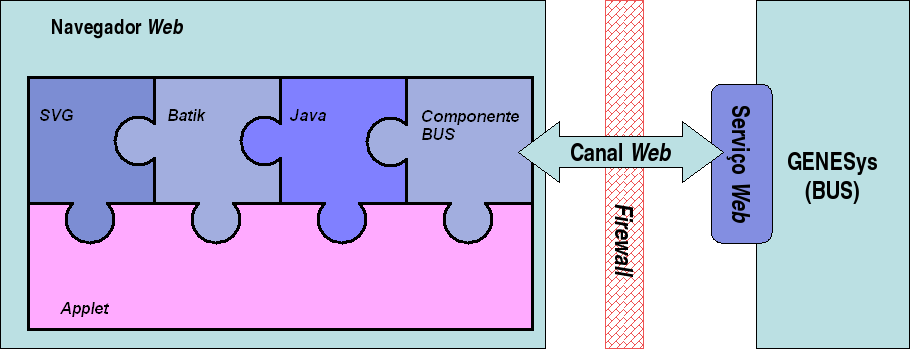
\includegraphics[width=0.86\textwidth]{puzzle}
    \caption{Arquitectura da Solução Proposta}
    \label{fig:arch}
  \end{center}
\end{figure}

Loren ipsum dolor sit amet, consectetuer adipiscing elit. 
Praesent sit amet sem. Maecenas eleifend facilisis leo. Vestibulum et
mi. Aliquam posuere, ante non tristique consectetuer, dui elit
scelerisque augue, eu vehicula nibh nisi ac est. Suspendisse elementum
sodales felis. Nullam laoreet fermentum urna. 

Duis eget diam. In est justo, tristique in, lacinia vel, feugiat eget,
quam. Pellentesque habitant morbi tristique senectus et netus et
malesuada fames ac turpis egestas. Fusce feugiat, elit ac placerat
fermentum, augue nisl ultricies eros, id fringilla enim sapien eu
felis. Vestibulum ante ipsum primis in faucibus orci luctus et
ultrices posuere cubilia Curae; Sed dolor mi, porttitor quis,
condimentum sed luctus. 

\subsection{Exemplo de Tabela}

É apresentado na Tabela~\ref{tab:exemplo1} um exemplo de tabela
flutuante e na Tabela~\ref{tab:exemplo2} um exemplo de tabela
flutuante, um pouco mais complicada.

\begin{table}[t]
  \centering
  \caption{Uma Tabela Simples}
\begin{tabular}{| l | p{45mm} |}
	\hline
\textbf{Acrónimo} & \textbf{Significado}\\
	\hline
	\hline
        ADT   & \emph{Abstract Data Type}\\\hline
        ANDF  & \emph{Architecture-Neutral Distribution Format}\\\hline
        API   & \emph{Application Programming Interface}\\
	\hline
\end{tabular}
  \label{tab:exemplo1}
\end{table}

Integer quis pede. Fusce nibh. Fusce nec erat vel mi condimentum
convallis. Sed at tortor non mauris pretium aliquet. In in lacus in
dolor molestie dapibus. Suspendisse potenti. Pellentesque sagittis
porta erat. Mauris sodales sapien id augue. Nam eu dolor. Donec sit
amet turpis non orci rhoncus commodo. Etiam condimentum commodo
libero.

Mauris pede. Curabitur faucibus dictum nibh. Proin tincidunt diam
vitae mauris. Sed hendrerit dolor vel ipsum. Nullam dapibus. Vivamus
tellus diam, egestas sit amet, vulputate non, vulputate id, eros. Nunc
sit amet nibh eget nibh imperdiet ornare. Cras vehicula mattis
ipsum. Sed diam arcu, semper at, gravida vitae, fermentum et,
nulla. Aenean massa orci, tristique nec, rutrum id, fringilla eget,
erat. Curabitur nulla ipsum, aliquam sed, rutrum vitae, semper quis,
ante. Fusce at nunc in dolor condimentum tempor. Duis sit amet massa. 

Curabitur convallis nulla quis risus. Nulla mollis porttitor
purus. Fusce ultricies odio at ligula pellentesque suscipit. Nulla
velit libero, blandit a, aliquet quis, hendrerit id, arcu. Phasellus
porttitor porttitor purus. Suspendisse velit tortor, fringilla sit
amet, commodo a, ultrices et, mi. Donec eu metus in erat ornare
adipiscing. Praesent varius mi ac nunc. Vestibulum leo lacus,
elementum in, vestibulum sit amet, hendrerit at, justo. Sed sit amet
neque. Donec libero risus, commodo sit amet, dignissim ut, tincidunt
a, eros. Ut non lacus quis tortor mattis ullamcorper. Vivamus
consequat augue vel erat. Sed tincidunt. Sed leo eros, ornare a,
pulvinar non, mattis quis, nibh. Aliquam faucibus mi ac nisi.

Pellentesque habitant morbi tristique senectus et netus et malesuada
fames ac turpis egestas. Duis aliquet, libero sit amet ornare viverra,
augue erat interdum dolor, vitae tincidunt lorem erat a lacus. Sed
lectus nisi, auctor in, hendrerit a, molestie vel, lectus. Cum sociis
natoque penatibus et magnis dis parturient montes, nascetur ridiculus
mus. Duis lacinia tempor dui. Vivamus rhoncus, tellus a viverra
dignissim, pede dui adipiscing odio, non faucibus metus mi gravida
eros. Nullam a tellus ut velit elementum tempus. Aenean rutrum
convallis tellus. Vestibulum nulla ante, dapibus ut, lobortis ut,
varius sed, nisl. Fusce lobortis. Sed ac lorem. Nulla tincidunt nulla
eget leo. Maecenas ac lectus eu neque ultrices pharetra. Curabitur a
risus nec arcu placerat tempor. Suspendisse magna nisl, viverra a,
adipiscing eget, ornare ultricies, ligula. Maecenas eu ligula vitae
eros convallis dignissim. 

\begin{table}[t]
  \centering
  \caption{Uma Tabela Mais Complicada}
\begin{tabular}{|c|r@{.}lr@{.}lr@{.}l||r|}
	\hline
\multicolumn{8}{|c|}
	{\rule[-3mm]{0mm}{8mm}Iteração $k$ de $f(x_n)$} \\
\textbf{\em k}
	& \multicolumn{2}{c}{$x_1^k$}
	& \multicolumn{2}{c}{$x_2^k$}
	& \multicolumn{2}{c||}{$x_3^k$}
	& comentários \\ \hline \hline
0   & -0&3                 & 0&6                 &  0&7   & - \\
1   &  0&47102965 & 0&04883157 & -0&53345964  & $\delta<\epsilon$ \\
2   &  0&49988691 & 0&00228830 & -0&52246185  & $\delta < \varepsilon$ \\
3   &  0&49999976 & 0&00005380 & -0&523656   &   $N$ \\
4   &  0&5                 & 0&00000307 & -0&52359743  & \\
\vdots	& \multicolumn{2}{c}{\vdots}
	& \multicolumn{2}{c}{$\ddots$}
	& \multicolumn{2}{c||}{\vdots}  & \\
7   &  0&5   & 0&0    & \textbf{-0}&\textbf{52359878}
		 & $\delta<10^{-8}$ \\ \hline
\end{tabular}
  \label{tab:exemplo2}
\end{table}

Loren ipsum dolor sit amet, consectetuer adipiscing elit. 
Praesent sit amet sem. Maecenas eleifend facilisis leo. Vestibulum et
mi. Aliquam posuere, ante non tristique consectetuer, dui elit
scelerisque augue, eu vehicula nibh nisi ac est. Suspendisse elementum
sodales felis. Nullam laoreet fermentum urna. 

Duis eget diam. In est justo, tristique in, lacinia vel, feugiat eget,
quam. Pellentesque habitant morbi tristique senectus et netus et
malesuada fames ac turpis egestas. Fusce feugiat, elit ac placerat
fermentum, augue nisl ultricies eros, id fringilla enim sapien eu
felis. Vestibulum ante ipsum primis in faucibus orci luctus et
ultrices posuere cubilia Curae; Sed dolor mi, porttitor quis,
condimentum sed luctus. 

\section{Secção Exemplo}

Loren ipsum dolor sit amet, consectetuer adipiscing elit. 
Praesent sit amet sem. Maecenas eleifend facilisis leo. Vestibulum et
mi. Aliquam posuere, ante non tristique consectetuer, dui elit
scelerisque augue, eu vehicula nibh nisi ac est. Suspendisse elementum
sodales felis. Nullam laoreet fermentum urna. 

Duis eget diam. In est justo, tristique in, lacinia vel, feugiat eget,
quam. Pellentesque habitant morbi tristique senectus et netus et
malesuada fames ac turpis egestas. Fusce feugiat, elit ac placerat
fermentum, augue nisl ultricies eros, id fringilla enim sapien eu
felis. Vestibulum ante ipsum primis in faucibus orci luctus et
ultrices posuere cubilia Curae; Sed dolor mi, porttitor quis,
condimentum sed luctus. 

\section{Resumo e Conclusões}

Resumir e apresentar as conclusões que se podem tirar no fim deste
capítulo.

\chapter{Implementação}\label{chap:chap4}

\section*{}

Este capítulo pode ser dedicado à apresentação de detalhes de nível
mais baixo relacionados com o enquadramento e implementação das
soluções preconizadas no capítulo anterior.
Note-se no entanto que detalhes desnecessários à compreensão do
trabalho devem ser remetidos para anexos.

Dependendo do volume, a avaliação do trabalho pode ser incluída neste
capítulo ou pode constituir um capítulo separado.

\section{Secção Exemplo}

%\todofigure{Inserir uma figura sobre o Map/Reduce}

Lorem ipsum dolor sit amet, consectetuer adipiscing elit. Integer
hendrerit commodo ante. Pellentesque nibh libero, aliquam at, faucibus
id, commodo a, velit. 
%\todoline{Escrever sobre o map/reduce}
Duis eleifend sem eget leo. Morbi in est. Suspendisse magna sem,
varius nec, hendrerit non, tincidunt quis, quam. Aenean congue. 
%\todolines{A short entry in the list of todos}{A very long todonote
%  that certainly will fill more than a single line in the list of
%  todos. Just to make sure let's add some more text.} 
Vivamus vel est sit amet sem iaculis posuere. Cras mollis, enim vel
gravida aliquam, libero nunc ullamcorper dui, ullamcorper sodales
lectus nulla sed urna. Morbi aliquet porta risus. 
Proin vestibulum ligula a purus. Maecenas a nulla. 
Maecenas mattis est vitae neque auctor tempus. Etiam nulla dui,
mattis vitae, porttitor sed, aliquet ut, enim. Cras nisl magna,
aliquet et, laoreet at, gravida ac, neque. Sed id est. Nulla dapibus
dolor quis ipsum rhoncus cursus. 

\section{Mais uma Secção}

Lorem ipsum dolor sit amet, consectetuer adipiscing elit. Quisque
purus sapien, interdum ut, vestibulum a, accumsan ullamcorper,
erat. Mauris a magna ut leo porta imperdiet. Donec dui odio, porta in,
pretium non, semper quis, orci. Quisque erat diam, pharetra vel,
laoreet ac, hendrerit vel, enim. Donec tristique luctus risus. Fusce
dolor est, eleifend id, elementum sit amet, varius vitae, neque. Morbi
at augue. Ut sem ligula, auctor vitae, facilisis id, pharetra non,
lectus. Nulla lacus augue, aliquam eget, sollicitudin sed, hendrerit
eu, leo. Suspendisse ac tortor. Mauris at odio. Etiam vehicula. Nam
lacinia purus at nibh. Aliquam fringilla lorem ac justo. Ut nec
enim. 
%\todoref{Citar Map/reduce}

Quisque ullamcorper. Aliquam vel magna. Sed pulvinar dictum
ligula. Sed ultrices dolor ut turpis. Vivamus sagittis orci malesuada
arcu venenatis auctor. Proin vehicula pharetra urna. Aliquam egestas
nunc quis nisl. Donec ullamcorper. Nulla purus. Ut suscipit lacus
vitae dui. Mauris semper. Ut eget sem. Integer orci. Nam vitae dui
eget nisi placerat convallis. 

\begin{lstlisting}[float,language=Java, label=src:mapreduce, caption=Example map and reduce functions for word counting]
map(String key, String value): 
// key: document name 
// value: document contents 
for each word w in value:
EmitIntermediate(w, "1");

reduce(String key, Iterator values):
// key: a word 
// values: a list of counts 
int result = 0;
for each v in values: 
result += ParseInt(v);

Emit(AsString(result))
\end{lstlisting}

Sed id lorem. Proin gravida bibendum lacus. Sed molestie, urna quis
euismod laoreet, diam dolor dictum diam, vitae consectetuer leo ipsum
id ante. Integer eu lectus non mauris pharetra viverra. In feugiat
libero ut massa. Morbi cursus, lorem sollicitudin blandit semper,
felis magna pellentesque lacus, ut rhoncus leo neque at tellus. Sed
mattis, diam eget eleifend tincidunt, ligula eros tincidunt diam,
vitae auctor turpis est vel nunc. In eu magna. Donec dolor metus,
egestas sit amet, ultrices in, faucibus sed, lectus. Etiam est enim,
vehicula pharetra, porta non, viverra vel, nunc. Ut non sem. Etiam nec
neque. 

\section{Resumo ou Conclusões}

Proin vehicula pharetra urna. Aliquam egestas
nunc quis nisl. Donec ullamcorper. Nulla purus. Ut suscipit lacus
vitae dui. Mauris semper. Ut eget sem. Integer orci. Nam vitae dui
eget nisi placerat convallis. 

\chapter{Conclusões e Trabalho Futuro} \label{chap:concl}

\section*{}

Deve ser apresentado um resumo do trabalho realizado e apreciada a
satisfação dos objetivos do trabalho, uma lista de contribuições
principais do trabalho e as direções para trabalho futuro.

A escrita deste capítulo deve ser orientada para a total compreensão
do trabalho, tendo em atenção que, depois de ler o Resumo e a
Introdução, a maioria dos leitores passará à leitura deste capítulo de
conclusões e recomendações para trabalho futuro.

\section{Satisfação dos Objetivos}

Lorem ipsum dolor sit amet, consectetuer adipiscing elit. Etiam non
felis sed odio rutrum ultrices. Donec tempor dolor. Vivamus justo
neque, tempus id, ullamcorper in, pharetra non, tellus. Praesent eu
orci eu dolor congue gravida. Sed eu est. Donec pulvinar, lectus et
eleifend volutpat, diam sapien sollicitudin arcu, a sagittis libero
neque et dolor. Nam ligula. Cras tincidunt lectus quis nunc. Cras
tincidunt congue turpis. Nulla pede velit, sagittis a, faucibus vitae,
porttitor nec, ante. Nulla ut arcu. Cras eu augue at ipsum feugiat
hendrerit. Proin sed justo eu sapien eleifend elementum. Pellentesque
habitant morbi tristique senectus et netus et malesuada fames ac
turpis egestas. Vivamus quam lacus, pharetra vel, aliquam vel,
volutpat sed, nisl. 

Nullam erat est, vehicula id, tempor non, scelerisque at,
tellus. Pellentesque tincidunt, ante vehicula bibendum adipiscing,
lorem augue tempor felis, in dictum massa justo sed metus. Suspendisse
placerat, mi eget molestie sodales, tortor ante interdum dui, ac
sagittis est pede et lacus. Duis sapien. Nam ornare turpis et
magna. Etiam adipiscing adipiscing ipsum. Fusce sodales nisl a
arcu. Cras massa leo, vehicula facilisis, commodo a, molestie
faucibus, metus. Suspendisse potenti. Duis sagittis. Donec porta. Sed
urna. Maecenas eros. Vivamus erat ligula, pharetra sit amet, bibendum
et, fermentum sed, dolor. Nullam eleifend condimentum nibh. Integer
leo nibh, consequat eget, mollis et, sagittis ac, felis. Duis viverra
pede in pede. Phasellus molestie placerat leo. Praesent at tellus a
augue congue molestie. Proin sed justo eu sapien eleifend
elementum. Pellentesque habitant morbi tristique senectus et netus et
malesuada fames ac turpis egestas. 

\section{Trabalho Futuro}

Lorem ipsum dolor sit amet, consectetuer adipiscing elit. Aliquam
tempor tristique risus. Suspendisse potenti. Fusce id eros. In eu
enim. Praesent commodo leo. Nullam augue. Pellentesque tellus. Integer
pulvinar purus a dui convallis consectetuer. In adipiscing, orci vitae
lacinia semper, sapien elit posuere sem, ac euismod ipsum elit tempus
urna. Aliquam erat volutpat. Nullam suscipit augue sed
felis. Phasellus faucibus accumsan est. 

Aliquam felis justo, facilisis sit amet, bibendum ut, tempus ac,
dolor. Sed malesuada. Nunc non massa. In erat. Nulla
facilisi. Phasellus blandit, est in accumsan cursus, libero augue
elementum leo, vitae auctor mauris nisl ac tortor. Cras porttitor
ornare elit. Fusce at lorem. Sed lectus tortor, vestibulum id, varius
a, condimentum nec, lectus. Maecenas in nisi et magna pretium
aliquam. Pellentesque justo elit, feugiat nec, tincidunt a, dignissim
vel, ipsum. Sed nunc. Vestibulum ante ipsum primis in faucibus orci
luctus et ultrices posuere cubilia Curae; Aliquam tempus rhoncus
leo. Donec neque quam, cursus sit amet, ultricies varius, semper non,
pede. Donec porttitor. Sed aliquet feugiat elit.  

\vspace*{12mm}

Lorem ipsum dolor sit amet, consectetuer adipiscing elit. Phasellus
tellus pede, auctor ut, tincidunt a, consectetuer in, felis. Mauris
quis dolor et neque accumsan pellentesque. Donec dui magna,
scelerisque mattis, sagittis nec, porta quis, nulla. Vivamus quis
nisl. Etiam vitae nisl in diam vehicula viverra. Sed sollicitudin
scelerisque est. Nunc dapibus. Sed urna. Nulla gravida. Praesent
faucibus, risus ac lobortis dignissim, est tortor laoreet mauris,
dictum pellentesque nunc orci tincidunt tellus. Nullam pulvinar, leo
sed vestibulum euismod, ante ligula elementum pede, sit amet dapibus
lacus tortor ac nisl. Morbi libero. Integer sed dolor ac lectus
commodo iaculis. Donec ut odio.  
 

%%----------------------------------------
%% Final materials
%%----------------------------------------

%% Bibliography
%% Comment the next command if BibTeX file not used, 
%% Assumes that bibliography is in ``myrefs.bib''
\PrintBib{myrefs}

%% Comment next 2 commands if numbered appendices are not used
\appendix
\chapter{Loren Ipsum} \label{ap1:loren}

Depois das conclusões e antes das referências bibliográficas,
apresenta-se neste anexo numerado o texto usado para preencher a
dissertação.

\section{O que é o \emph{Loren Ipsum}?}

\emph{\textbf{Lorem Ipsum}} is simply dummy text of the printing and
typesetting industry. Lorem Ipsum has been the industry's standard
dummy text ever since the 1500s, when an unknown printer took a galley
of type and scrambled it to make a type specimen book. It has survived
not only five centuries, but also the leap into electronic
typesetting, remaining essentially unchanged. It was popularised in
the 1960s with the release of Letraset sheets containing Lorem Ipsum
passages, and more recently with desktop publishing software like
Aldus PageMaker including versions of Lorem Ipsum~\citep{kn:Lip08}. 

\section{De onde Vem o Loren?}

Contrary to popular belief, Lorem Ipsum is not simply random text. It
has roots in a piece of classical Latin literature from 45 BC, making
it over 2000 years old. Richard McClintock, a Latin professor at
Hampden-Sydney College in Virginia, looked up one of the more obscure
Latin words, consectetur, from a Lorem Ipsum passage, and going
through the cites of the word in classical literature, discovered the
undoubtable source. Lorem Ipsum comes from sections 1.10.32 and
1.10.33 of ``de Finibus Bonorum et Malorum'' (The Extremes of Good and
Evil) by Cicero, written in 45 BC. This book is a treatise on the
theory of ethics, very popular during the Renaissance. The first line
of Lorem Ipsum, ``Lorem ipsum dolor sit amet\ldots'', comes from a line in
section 1.10.32.

The standard chunk of Lorem Ipsum used since the 1500s is reproduced
below for those interested. Sections 1.10.32 and 1.10.33 from ``de
Finibus Bonorum et Malorum'' by Cicero are also reproduced in their
exact original form, accompanied by English versions from the 1914
translation by H. Rackham.

\section{Porque se usa o Loren?}

It is a long established fact that a reader will be distracted by the
readable content of a page when looking at its layout. The point of
using Lorem Ipsum is that it has a more-or-less normal distribution of
letters, as opposed to using ``Content here, content here'', making it
look like readable English. Many desktop publishing packages and web
page editors now use Lorem Ipsum as their default model text, and a
search for ``lorem ipsum'' will uncover many web sites still in their
infancy. Various versions have evolved over the years, sometimes by
accident, sometimes on purpose (injected humour and the like). 

\section{Onde se Podem Encontrar Exemplos?}

There are many variations of passages of Lorem Ipsum available, but
the majority have suffered alteration in some form, by injected
humour, or randomised words which don't look even slightly
believable. If you are going to use a passage of Lorem Ipsum, you need
to be sure there isn't anything embarrassing hidden in the middle of
text. All the Lorem Ipsum generators on the Internet tend to repeat
predefined chunks as necessary, making this the first true generator
on the Internet. It uses a dictionary of over 200 Latin words,
combined with a handful of model sentence structures, to generate
Lorem Ipsum which looks reasonable. The generated Lorem Ipsum is
therefore always free from repetition, injected humour, or
non-characteristic words etc. 


%% Index
%% Uncomment next command if index is required, 
%% don't forget to run ``makeindex mieic'' command
%\PrintIndex

\end{document}
